% Complete implicit suffix tree for abbbc; all five suffixes end at leaves.
% Node 5 splits the root edge at b; nodes 6 and 7 represent bc and c.
% Regenerate from this directory:
% latex -interaction=nonstopmode -halt-on-error suffix-tree7.tex
% dvisvgm --no-fonts --exact --bbox=papersize -o suffix-tree7.svg suffix-tree7.dvi
\documentclass[tikz,border=8pt]{standalone}
\usepackage{lmodern}
\usetikzlibrary{arrows.meta}
\definecolor{nodecolor}{HTML}{242A31}
\begin{document}
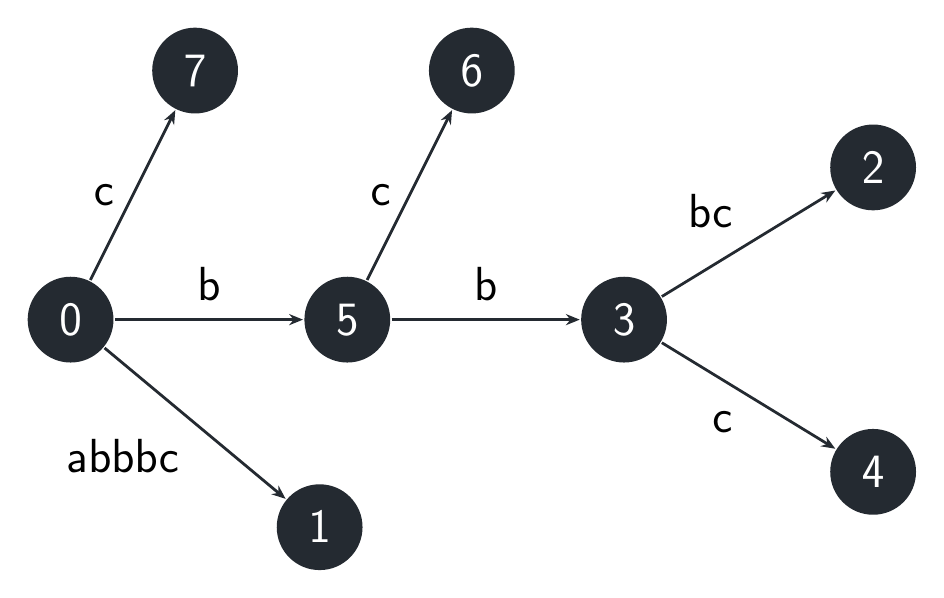
\begin{tikzpicture}[
  x=1pt,y=-1pt,line width=1pt,draw=nodecolor,
  font=\sffamily\fontsize{18}{21}\selectfont,
  vertex/.style={circle,fill=nodecolor,text=white,minimum size=31pt,inner sep=0pt},
  every edge/.style={draw,-{Stealth[length=5pt,width=4pt]}}
]
  \node[vertex] (n0) at (0,0) {0};
  \node[vertex] (n1) at (90,75) {1};
  \node[vertex] (n2) at (290,-55) {2};
  \node[vertex] (n3) at (200,0) {3};
  \node[vertex] (n4) at (290,55) {4};
  \node[vertex] (n5) at (100,0) {5};
  \node[vertex] (n6) at (145,-90) {6};
  \node[vertex] (n7) at (45,-90) {7};
  \path
    (n0) edge node[below left=2pt] {abbbc} (n1)
    (n0) edge node[above=3pt] {b} (n5)
    (n0) edge node[left=3pt] {c} (n7)
    (n5) edge node[above=3pt] {b} (n3)
    (n5) edge node[left=3pt] {c} (n6)
    (n3) edge node[above left=2pt] {bc} (n2)
    (n3) edge node[below left=2pt] {c} (n4);
\end{tikzpicture}
\end{document}
